%!TEX root = ../Report.tex

In this chapter of the report, we discuss the results of the experiments and their ramifications. The structure of this section mirrors that of the experiments section, so that the first results discussed will be the first experiment detailed in chapter \ref{chapter:experimental_methodology_and_program}.



\section{Experiment Results}



\subsection{Experiment 1 - Metrics Collection Overhead}

Runtime without metrics: 67862.0
Runtime with metrics:    68047.0

(*** Should I make this a graph? ***)

185ms of delay, 0.003\% of total runtime.

\begin{figure}
	\centering
	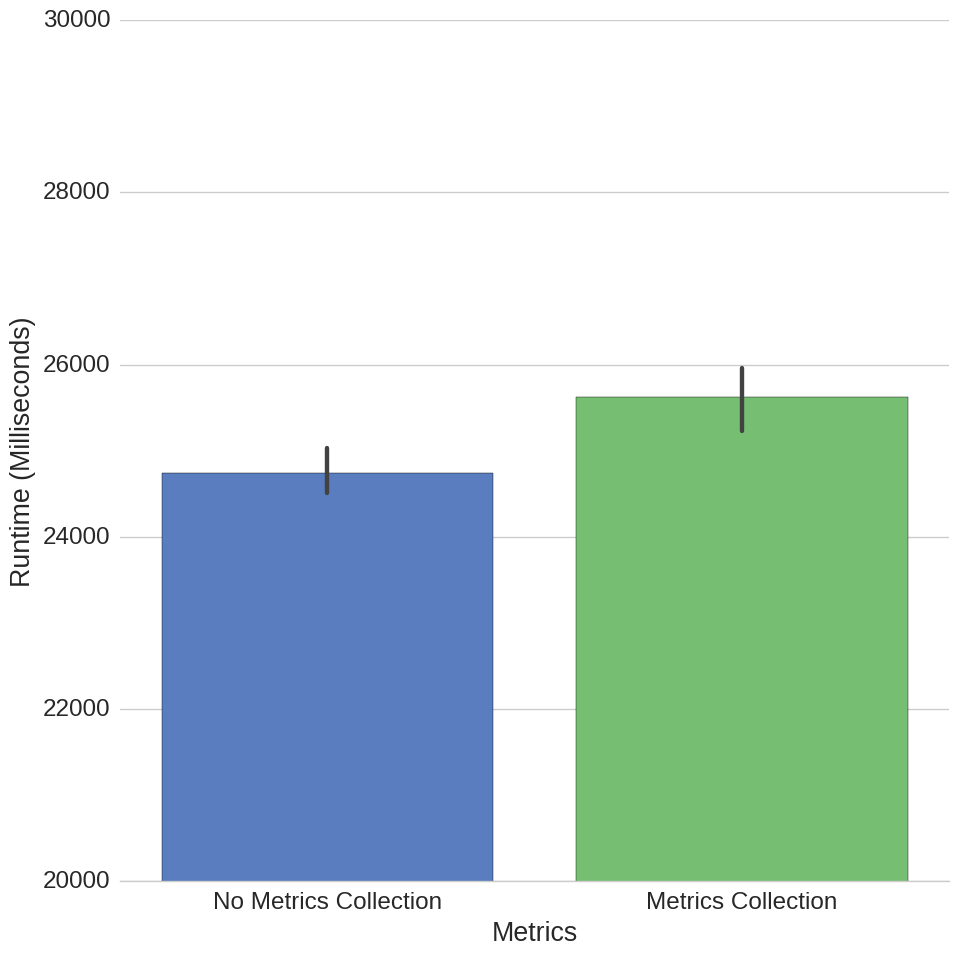
\includegraphics[width=\textwidth]{graphics/experiment1.png}
	\caption{Experiment 1 results}
	\label{fig:results_ex1}
\end{figure}

%% LaTeX2e file `ex_params/ex1_params.tex'
%% generated by the `filecontents' environment
%% from source `Report' on 2017/03/25.
%%
\begin{table}
\centering
 \begin{tabular}{|c|c|}
  \hline
  Number of tasks & 100,000 \\
  \hline
  Task Grain & 100,000 Repeats \\
  \hline
  Task Grain Distribution & Uniform \\
  \hline
  Number of CPU cores & 4 \\
  \hline
  Number of threads used & 4 \\
  \hline
  Thread pinning & Uniform \\
  \hline
  Schedule & Dynamic Chunks (Chunk Size = 1000) \\
  \hline
 \end{tabular}
\caption{Experiment 1 Parameters}
\iflabela
\label{table:evaluation_ex1_parameters}
\fi
\labelatrue
\end{table}




\subsection{Experiment 2 - Absolute Performance}

In this experiment, the total run times of three implementations are measured. One sequential implementation, a standard modern parallel implementation utilizing OMP, and our plastic implementation. Our plastic implementation is running with no plasticity for the moment, and with no messaging functionality at all. This is so it is comparable to a standard parallel implementation.

The OMP and our implementation are using a dynamic chunks schedule, with a chunk size of 500. All programs were compiled at optimization level 3.

Fig. \ref{fig:results_ex2} shows us that with a single thread, our performance is similar to a sequential implementation, and as we increase the thread count, our performance scales accordingly. Overall, this shows that our baseline implementation performs on a par with current parallel implementations, providing a good baseline performance. 

\begin{figure}
	\centering
	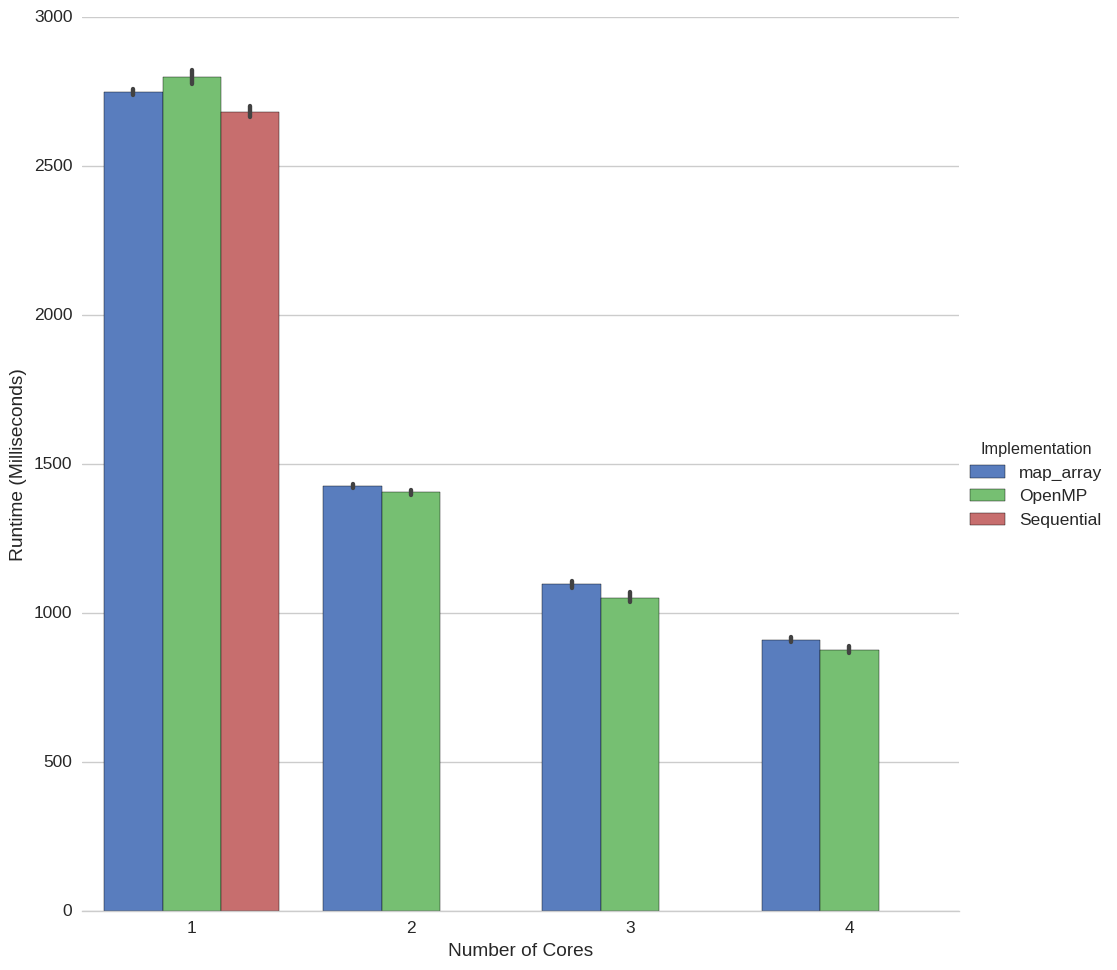
\includegraphics[width=\textwidth]{graphics/experiment2.png}
	\caption{Experiment 2 results}
	\label{fig:results_ex2}
\end{figure}

%% LaTeX2e file `ex_params/ex2_params.tex'
%% generated by the `filecontents' environment
%% from source `Report' on 2017/03/25.
%%
\begin{table}
\centering
 \begin{tabular}{|c|c|c|c|}
  \hline
  Number of tasks & 10,000 \\
  \hline
  Task Grain & 1,000,000 Repeats \\
  \hline
  Task Grain Distribution & Uniform \\
  \hline
  Number of CPU cores & 4 \\
  \hline
  Number of threads used & \specialcell{1, \\ 2, \\ 3, \\ 4} \\
  \hline
  Thread pinning & Uniform \\
  \hline
  Schedule & Static \\
  \hline
 \end{tabular}
\caption{Experiment 2 Parameters}
\iflabelb
\label{table:evaluation_ex2_parameters}
\fi
\labelbtrue
\end{table}




\subsection{Experiment 3 - Plasticity And Contention Aware Scheduling Framework Overhead}


Results:

Runtime without plasticity etc: 24153.0
Runtime with plasticity etc:    24684.0

Standard deviation!

(*** Should I make this a graph? Yes - different input sizes***)

531ms of delay, 0.02\% of total runtime.

\begin{figure}
	\centering
	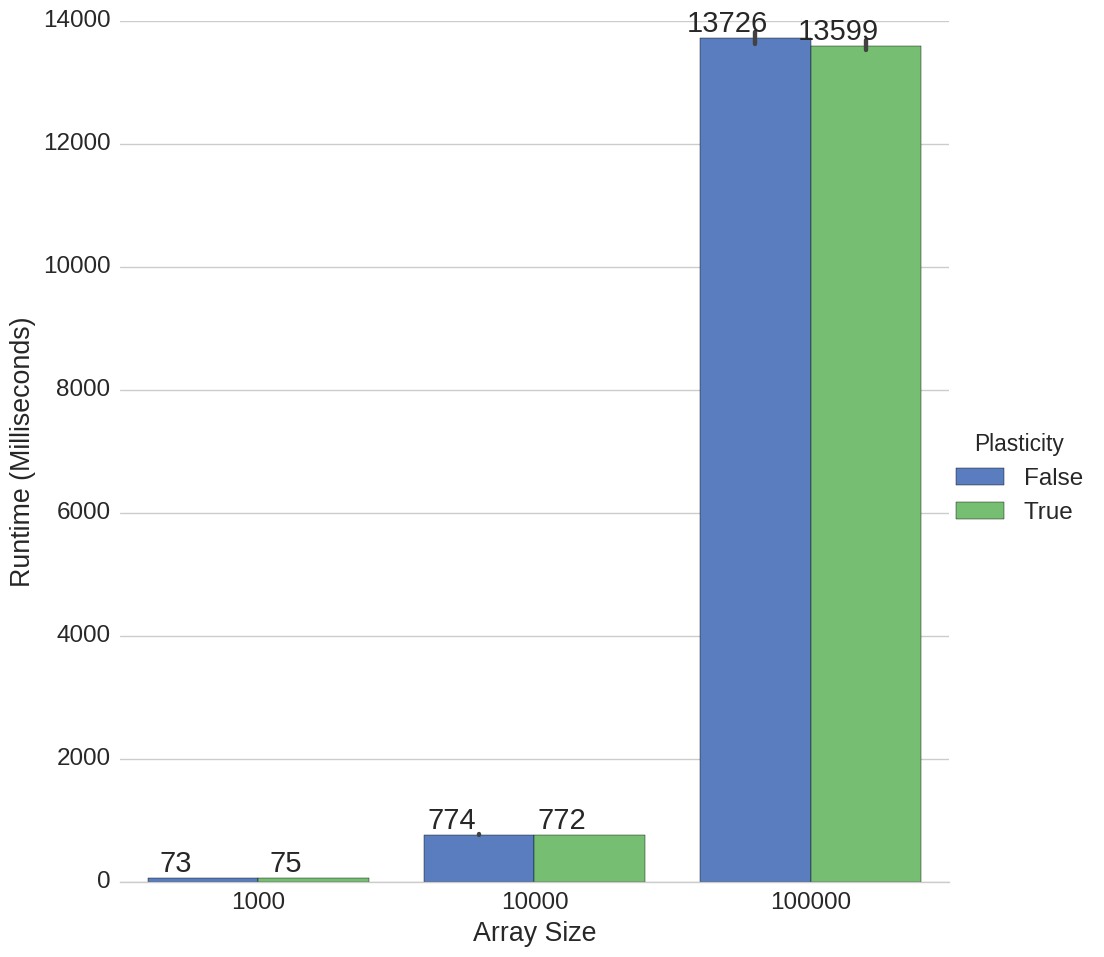
\includegraphics[width=\textwidth]{graphics/experiment3.png}
	\caption{Experiment 3 results}
	\label{fig:results_ex3}
\end{figure}

%% LaTeX2e file `ex_params/ex3_params.tex'
%% generated by the `filecontents' environment
%% from source `Report' on 2017/03/25.
%%
\begin{table}
\centering
 \begin{tabular}{|c|c|}
  \hline
  Number of tasks & 100,000 10,000 1,000 \\
  \hline
  Task Grain & Medium \\
  \hline
  Task Grain Distribution & Uniform \\
  \hline
  Number of CPU cores & 4 \\
  \hline
  Number of threads used & 4 \\
  \hline
  Thread pinning & Uniform \\
  \hline
  Schedule & Dynamic Chunks \\
  \hline
 \end{tabular}
\caption{Experiment 3 Parameters}
\iflabelc
\label{table:evaluation_ex3_parameters}
\fi
\labelctrue
\end{table}




\subsection{Experiment 4 - Schedule Choice Importance}

\begin{figure}
	\centering
	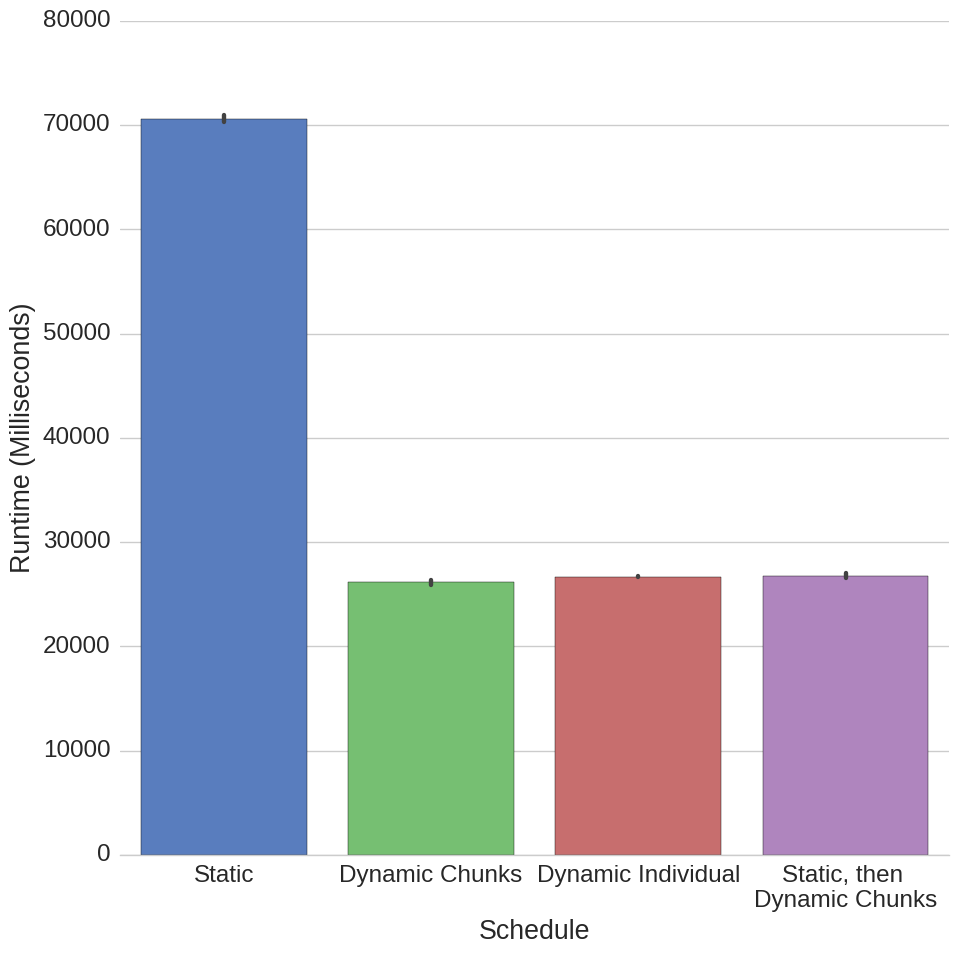
\includegraphics[width=\textwidth]{graphics/experiment4.png}
	\caption{Experiment 4 results}
	\label{fig:results_ex4}
\end{figure}

%% LaTeX2e file `ex_params/ex4_params.tex'
%% generated by the `filecontents' environment
%% from source `Report' on 2017/03/25.
%%
\begin{table}
\centering
 \begin{tabular}{|c|c|}
  \hline
  Number of tasks & 100,000 \\
  \hline
  Task Grain & Large and small \\
  \hline
  Task Grain Distribution & Biased \\
  \hline
  Number of CPU cores & 4 \\
  \hline
  Number of threads used & 4 \\
  \hline
  Thread pinning & Uniform \\
  \hline
  Schedule & \specialcell{Static, \\ Dynamic Chunks (Chunk Size = 1,000), \\ Dynamic Chunks (Chunk Size = 1) \\ Static, then dynamic chunks after 5 seconds} \\
  \hline
 \end{tabular}
\caption{Experiment 4 Parameters}
\iflabeld
\label{table:evaluation_ex4_parameters}
\fi
\labeldtrue
\end{table}




\subsection{Experiment 5 - Absolute Multiprogramming Performance}

%% LaTeX2e file `ex_params/ex5_params.tex'
%% generated by the `filecontents' environment
%% from source `Report' on 2017/03/25.
%%
\begin{table}
\centering
 \begin{tabular}{|c|c|}
  \hline
  Program 1 & \\
  \hline
  Number of tasks & 30,000 \\
  \hline
  Task Grain & 10,000,000 Repeats \\
  \hline
  Task Grain Distribution & Uniform \\
  \hline
  Number of CPU cores & 4 \\
  \hline
  Number of threads used & \specialcell{4 \\ 4, then 2, then 4} \\
  \hline
  Thread pinning & \specialcell{Loose, \\ Uniform} \\
  \hline
  Schedule & Dynamic\_individual \\
  \hline
 \end{tabular}

 \begin{tabular}{|c|c|}
  \hline
  Program 2 & \\
  \hline
  Number of tasks & 15,000 \\
  \hline
  Task Grain & 10,000,000 Repeats \\
  \hline
  Task Grain Distribution & Uniform \\
  \hline
  Number of CPU cores & 4 \\
  \hline
  Number of threads used & \specialcell{4 \\ 2} \\
  \hline
  Thread pinning & \specialcell{Loose, \\ Uniform} \\
  \hline
  Schedule & Dynamic\_individual \\
  \hline
 \end{tabular}
\caption{Experiment 5 Parameters}
\iflabele
\label{table:evaluation_ex5_parameters}
\fi
\labeletrue
\end{table}




\section{Discussion}

 ***Discuss the findings of the results, (Mention weird runtimes with many small tasks!)***